% !TEX TS-program = pdflatex
% !TEX encoding = UTF-8 Unicode
 
\documentclass[12pt]{report} % use larger type; default would be 10pt
 
\usepackage[utf8]{inputenc} % set input encoding (not needed with XeLaTeX)
 
%%% Examples of Article customizations
% These packages are optional, depending whether you want the features they provide.
% See the LaTeX Companion or other references for full information.
 
%%% PAGE DIMENSIONS
\usepackage{geometry} % to change the page dimensions
\geometry{a4paper} % or letterpaper (US) or a5paper or....
\geometry{margin=1in} % for example, change the margins to 2 inches all round
\geometry{landscape} % set up the page for landscape
%read geometry.pdf for detailed page layout information
 
\usepackage{graphicx} % support the \includegraphics command and options
 
% \usepackage[parfill]{parskip} % Activate to begin paragraphs with an empty line rather than an indent
 
%%% PACKAGES
\usepackage{booktabs} % for much better looking tables
\usepackage{array} % for better arrays (eg matrices) in maths
\usepackage{paralist} % very flexible & customisable lists (eg. enumerate/itemize, etc.)
\usepackage{verbatim} % adds environment for commenting out blocks of text & for better verbatim
\usepackage{subfig} % make it possible to include more than one captioned figure/table in a single float
\usepackage{amsmath}
\usepackage{gensymb}
% These packages are all incorporated in the memoir class to one degree or another...
 \graphicspath{{Figures/}}
%%% HEADERS & FOOTERS
\usepackage{fancyhdr} % This should be set AFTER setting up the page geometry
\pagestyle{fancy} % options: empty , plain , fancy
\renewcommand{\headrulewidth}{0pt} % customise the layout...
\lfoot{}\cfoot{\thepage}
 
\rfoot{}
 
%%% SECTION TITLE APPEARANCE
\usepackage{sectsty}
\allsectionsfont{\sffamily\mdseries\upshape} % (See the fntguide.pdf for font help)
% (This matches ConTeXt defaults)
 
 
%%% END Article customizations
 
%%% The "real" document content comes below...
 
\title{\bf Flying Carpet Scale Model Testing\\  }
\author{\bf Micaiah Smith-Pierce
\\ Experimental Aerodynamics and Concepts Group
\\Daniel Guggenheim School of Aerospace Engineering
\\Georgia Institute of Technology
\\Atlanta GA 30332-0150
}
\date{\it Updated 30 April, 2018} % Activate to display a given date or no date (if empty),
 
         % otherwise the current date is printed 

\usepackage{graphicx}
 
\begin{document}
\maketitle
 
\tableofcontents
 
\chapter{Abstract}

Designs for the a Flying Carpet Glitter Belt aircraft were considered and wind tunnel models were tested. Different schemes for reducing flutter
were devised and tested. These included
reinforcing the sheet with rigid structures along its edges, holding the sheet under tension by its corners, changing the shape of the
sheet, adding wires under tension to its edges, taping it continously along its lateral edges, and cutting small holes in the sheet.
Some lift data was obtained. The best method of
reducing flutter was found to be suspending the sheet under tension by its four corners, making the edges of the sheet to be concavely
parabolic in shape, and attaching threads under high tension to the leading and trailing edges. Lift and drag data for this configuration was
obtained.

\chapter{Introduction}

The Glitter belt project aims to reverse climate change by reflecting solar radiation out to space.  The reflection will be accomplished
by solar-powered aicraft carrying ultralight mylar sheets at approximately 100,000 feet of altitude.  Cost analysis shows that this is
feasible to do using government funding.  The name "Glitter Belt" refers to the appearance the reflectors may have when viewed from space.

There are three different concepts for implementing the Glitter Belt: The Flying Carpet, the Quadrotor, and the Baloon Beanie.  The
author's work concerns primarily the first, which includes more challenging aerdynamic questions,
appropros of this lab group's title and purpose.  In the Flying Carpet,
the first, the mylar sheet is supported by aerodynamic lift.  During the day, it is towed through the air by propellers, driven
by electric motors.  The propellers are mounted on a flying wing, and the motors are powered by solar cells on the wing.  During the
night, the aircraft maintains forward flight by gliding downward, using gravitatational potential energy, staying above the upper limit
of controlled airspace, 60,000 feet.  Incidentally, this concept may also be useful for transportation on Mars, since the martian atmosphere
at lower altitude is similar to that of earth at 100,000 feet.
\begin{figure}
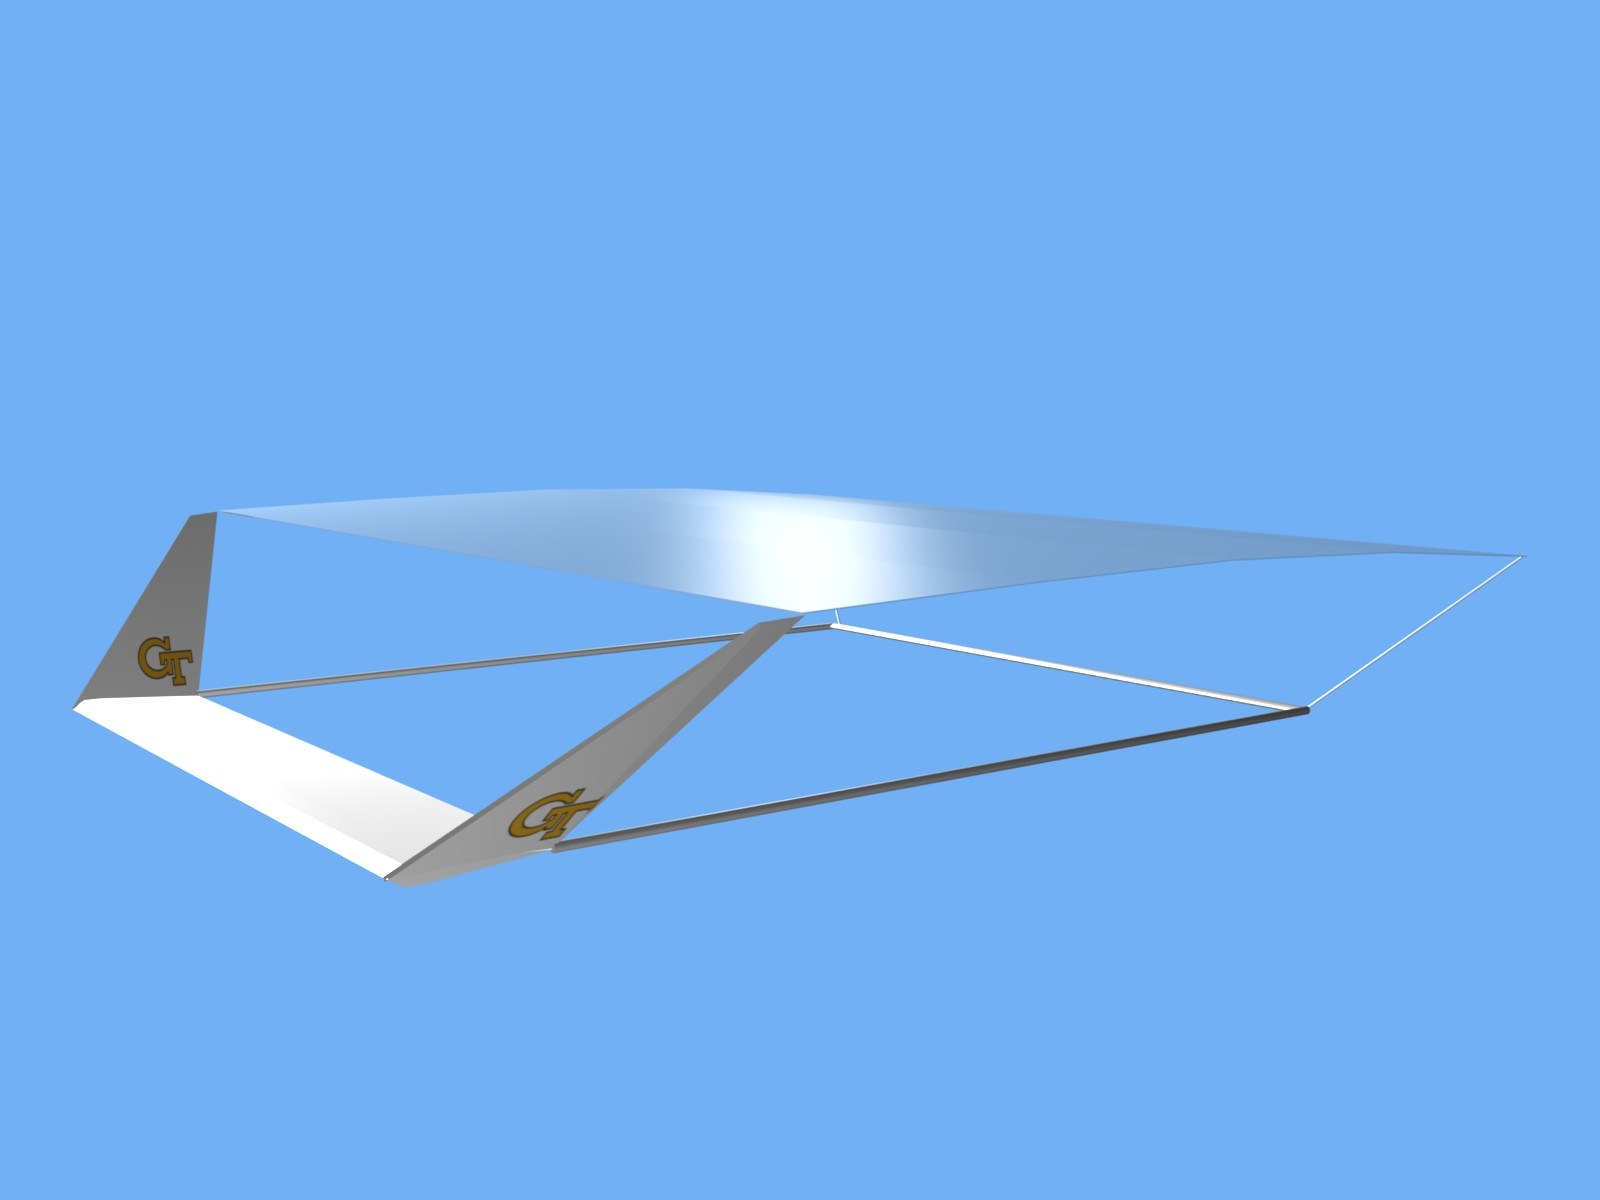
\includegraphics[width = 10cm]{FlyingCarpet.jpg}
\caption{An artist's concept of the Flying Carpet}
\end{figure}

The second concept is the Quadrotor.  This involves supporting the sheets using four rotary wings.  Thus far no feasible way has been
found to keep such an aircraft above 60,000 feet at night, so the author's work is not concerned with it.

The third and final concept is the Balloon Beanie.  In this concept, a flat reflector sheet is supported by hydrogen balloons.  Some
solar powered rotors are included to provide trim and propulsion. (It will be necessary under certain conditions to move the aircraft,
although most of the time it will drift in the wind.)  This may be particularly useful near the poles, where due to the low angle of
elevation of the sun, a horizontal reflector such as the Flying Carpet will be less effective.
and the later nearer to the equator.

\chapter{Define Objectives}
 

{\bf Objectives:}
\begin{itemize}
	\item Build a model of the Flying Carpet, approximately 70cm in span,which can:
	\begin{itemize}
		\item carry a reflector sheet internally, as in the climb phase of the mission
		\item deploy the sheet
		\item hold the sheet steady (without significant flutter) during a wind tunnel test
	\end{itemize}
	\item Obtain lift and drag data for this model
\end{itemize}

\chapter{Prior Work}

Cost analysis shows that the Glitter Belt project can be implimented using government expenditures.  It also shows that the flying carpet
will probably be cheaper to produce per unit reflector area than the Balloon Beanie.  However, the Balloon Beanie has the unique property
of being capable of orienting to be normal to the Sun's rays no matter the angle.  This eliminates the need to place them on the part of
the Earth directly beneath the Sun, near the poles in particular (for the purpose of stopping ice melting).  The author suggests that
both concepts may be manufactured, and the Flying Carpet may be deployed beneath the Sun and the Balloon Beanie may be deployed near the
poles.

The primary challenge of the Flying Carpet concept is keeping the reflector sheet smooth and flat.  Present design calls for a sheet
of reflective mylar trailing behind the wing.  However, wind tunnel testing has shown that the sheet oscillates in a self-excited manner.
 When the aspect ratio is high, the oscillations propagate spanwise.  When the aspect ratio is low (i.e. less than 1) the oscillations
are longitudinal.  Moving the sheet away from the wing, or making spanwise slits in it does not help.  Limited success has been achieved
by introducing rigid structures made of drinking straws into the sheet.  The oscillations are detrimental in that they increase drag
and reduce the effective area of the sheet.

Another design calls for stretching the sheet by its four corners which will be connected to a rigid frame.  This causes a problem because
the sheet bends upward like a parachute, which has inferior aerodynamic and reflective characteristics.

\chapter{Project Schedule}
\begin{itemize}
  \item Friday 1-19-18:  Discussed concepts for a Glitter Belt model
  \item Monday 1-22-18:  Designed a base for the Glitter Belt model, consisting of a wing, (where the engines and solar cells would
reside, and two winglets which could be installed at different dihedral and sweepback angles.
  \item Friday 1-26-18:  Constructed base of model
  \item Monday 1-29-18:
  \begin{itemize}
    \item installed PVC pipe and paper to form respectively the leading and trailing edge of the base wing
    \item installed sheet tail booms
    \item began construction of trailing edge airfoil
  \end{itemize}
  \item Friday 2-2-18
  \begin{itemize}
    \item Finished construction of trailing edge airfoil.
    \item Installed sheet and trailing edge airfoil
    \item discussed concepts for a deployable sheet
  \end{itemize}
  \item Monday morning 2-5-18:  Show existing model to Prof. Komerath and obtain directives for further development/testing
  \item Monday afternoon 2-5-18:
  \begin{itemize}
    \item test Prof. Komerath's idea to dampen flutter using holes in the sheet
    \item construct proof of concept for wire-constraint idea
  \end{itemize}
  \item Friday 2-9-18:
  \begin{itemize}
    \item build and test wire-constrained model
  \end{itemize}
  \item Monday 2-12-18:
  \begin{itemize}
    \item obtain next goal from Prof. K.
  \end{itemize}
  \item Friday 2-16-18:  Measure Low Turbulence Wind Tunnel mount and fan blade and create CAD drawing
  \item Monday 2-19-18 through Monday 2-26-18:  Wait for TAs in charge of the Low Turbulence Wind Tunnel to
fix a software issue so that testing may begin.
  \item Thursday 3-1-18 and Friday 3-2-18:  Test fan blade as a flat plate airfoil in order to gain proficiency using
the wind tunnel and assist the AE 1601 classes.
  \item Friday 3-9-17 through Friday 3-16-18:  Test Flying Carpet in the wind tunnel.
	\item Monday 3-19-18: Test Flying Carpet using mylar sheet
	\item Friday 3-23-18: Attempt to validate lift-weight stability theory in wind tunnel
	\item Friday 4-6-18 and Monday 4-9-17: Prepare poster for Undergraduate Research Fair
	\item Tuesday 4-10-18: Present research at Undergraduate Research Fair
	\item Friday 4-13-18 and Monday 4-16-18: Build Tension Concept Version 4
	\item Friday 4-17-18 Perform rudimentary testing of TC V.4 as time and wind tunnel access allows
\end{itemize}

\chapter{Experimental Setup}

The model underwent preliminary testing using the John Harper wind tunnel's ventilation fan in order to visually confirm that
techniques form minimizing sheet flutter are effective.  The sheet will be rigorously tested in the Low Turbulence wind tunnel.

\subsection{Model Details}

The model consists of a base wing, winglets, a sheet, and a trailing edge airfoil.  The wing is made out of a styrofoam block.
 It has a PVC pipe taped to the leading edge and two sheets of paper which are attatched to the rear face of the styrofoam
block and join together to form a sharp trailing edge.  Two winglets were laser cut out of plywood.  There are two holes in the end of
the base wing and a ring of holes in each winglet.  A threaded pin fits through the holes in the base wing and through a pair of holes
in each winglet.  The each connection is secured by a total of four nuts.  By using pins which are bent at different angles, any dihedral
can be achieved, and by selecting a different pair of holes in the winglets, any sweepback angle can be achieved.

The sheet and trailing edge airfoil have gone through several iterations, described below.

\subsubsection{Simple (Original) Version}
The sheet is supported by two tail booms, constructed from drinking straws, which are attatched to the tips of the winglets using hot
glue.  The sheet, made of heat-shrink plastic, is taped to the tail booms.  A high aspect ratio wing, made by sanding styrofoam until
its cross section resembled an airfoil, was glued to the rear end of the tail booms.  This is referred to tas the trailing edge airfoil.
 The trailing edge of the sheet is taped to the upper surface of the trailing edge airfoil.

\subsubsection{Deployable Sheet Concept}
In the full scale prototype, the trailing edge airfoil is intended to be used to maintain the trim of the sheet.  There will be actuators
which manipulate its AOA.  Also in the full scale prototype, the sheet must be contained internally during takeoff and the climb to
100000 feet and be deployed at said alititde.  Our model must simulate this, and several concepts have been discussed:
\begin{itemize}
  \item The sheet may start out rolled up inside the base wing and be dragged into position by means of a pulley system, operated by
a pair of servo motors inside the wing.
  \item The sheet may start out rolled up inside the trailing edge airfoil.  The trailing edge airfoil would be connected to the tail booms
which would be mounded on a pair of servo actuators mounted on the winglets.  The sheet would be attatched to the winglets, such that at
cruise altitude, the sevos would move the tail booms and trailing edge airfoil back, and the sheet would unroll.
  \item The tail booms may be "telescoping", i.e. made of multiple subsections, which may fit inside one another to dramatically decrease
the overal lengeth.  At altitude, the trailing edge airfoil would increase its AOA past stall, and the aerodynamic drag would pull the
trailing edge airfoil back into position, extending the tail booms and unrolling the sheet.
\end{itemize}

This concept has not yet been built

\subsubsection{Dampening Holes}
In hopes of dampening the oscillations, six holes were cut in the sheet, each approximately 1cm in diameter (Figure \ref{fig:damp}).  The rationale behind these
holes is as follows:  Assume the sheet is oscillating in a pattern that can be modeled by the 2D wave equation.  Allowing air to flow
through holes in the sheet should either reduce the forcing due to aerodynamic forces or provide a damping force in the form of drag.
 Thus, the holes were cut at the locations where the greatest amplitude of oscillation was observed, presumably the antinodes.
\begin{figure}
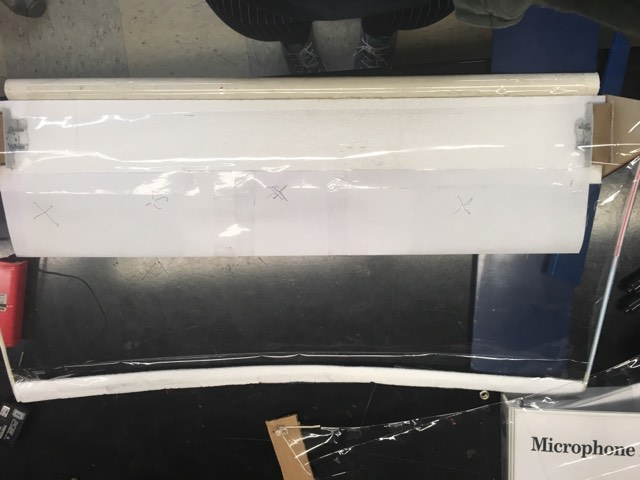
\includegraphics[width = 10cm]{gb_simple_version.jpg}
\caption{The dampening holes model.  A hole is located at the center of each "X" drawn on the sheet.}
\label{fig:damp}
\end{figure}

\subsubsection{Wire Constraints (Tension Concept Version 1)}
See figure \ref{fig:wire}.  Cardboard strips were glued on top of the tail booms (so far made of straws) and trailing edge airfoil to
stiffen them.  Four pieces of
thin electrical wire were tied to a piece of a rubber band at each end using a triple overhand knot.  The rubber bands were glued
to the winglets and the ends of the trailing edge airfoil so that the wires formed a rectangle.  The wire-rubber band assemblies are
of such a length that when in place on the model they are under a small amount of tension.

A 71cm by 35.5cm rectangular sheet was cut as before.  However, four additional cuts were made.  Each cut was in the shape of a parabola.
 The parabolic cuts on the two long edges had a vertex 5cm behind (toward the center of the sheet) the corners of the sheet, and the cuts
on the short edges were correspondingly 2.5cm deep.  Thus the sheet has edges which bow inward, so that it vaguely resembles a star.  In
order to attatch the sheet to the model, the sheet was taped to the wires at roughly 5cm intervals.  Because the wires are under tension,
the sheet is now under tension.
\begin{figure}
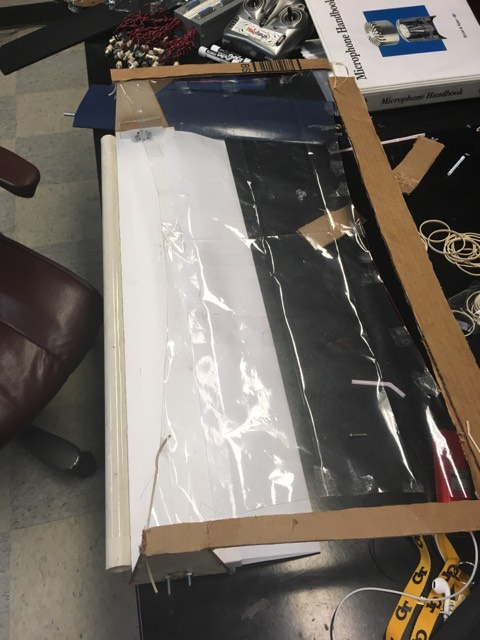
\includegraphics[height = 10cm]{gb_wire_constraint.jpg}
\caption{The wire-constrained model}
\label{fig:wire}
\end{figure}

There is a reason behind the parabolic shape of the cuts.  The sheet is to be under uniform tension, so the wire must support a uniformly
distributed load.  Consider the wire on the leading edge of the sheet, using standard vehicle-centered aeronautical coordinated (i.e. the
x-axis is roughly parallel to the chord line, the y-axis is roughly parallel to the leading edge, and the z-axis points toward the ground).
 Let the contour followed by the wire be given by
\[x = f(y)\]
and the tension be $T(y)$, which may be resolved into components $T_x(y)$ and $T_y(y)$.  Clearly,
\[\frac{T_x}{T_y} = \frac{\partial f}{\partial y}\]
Now, consider the small segment of the wire at $y_1$ with lenth $dy$.  In order for it to be in equilibrium, we have
\[T_y(y_1) - T_y(y_1 + dy) = 0\],
i.e. $T_y$ is constant throughout the wire.  Furthermore, since the sheet is under uniform tension, there will be some uniform distributed
load $\lambda$ on the wire, i.e. for any points $y_a$ and $y_b$, the sheet exerts a force on the segment of wire between $y_a$ and $y_b$
equal to
\[\lambda |y_a - y_b|\]
in the negative $x$ direction.  The upward force due to the tension in the wire must equal this force, so we have
\[T_x(y_1) - T_x(y1 + dy) = \lambda*dy\]
\[\frac{T_x(y_1) - T_x(y1 + dy)}{dy} = \lambda\]
\[\frac{\partial T_x}{\partial y}(y1) = \lambda\]
\[\frac{\partial^2 f}{\partial y^2} = \frac{\lambda}{T_y}\].
Integrating,
\[f(y) = \lambda y^2 + Cy + D\]
for some constants $C$ and $D$.  This shows that $f$ is quadratic, so a parabola is the correct shape for a wire to hold up a sheet under
uniform tension.  The same shape can be observed in some suspension bridges.

Furthermore, because the fluttering appeared to occur in spots where the sheet was loose, one may speculate that putting the sheet under
uniform tension may eliminate all loose places ad thus eliminate the flutter instability.

\subsubsection{Tension Concept Version 2}

In the Wire Constraints/TCV 1 model, a wire was used to put the sheet under uniform tension.  However, it was hypothesized that if the wire
was removed, the same flutter reduction may be achieved (even though the tension may not be uniform).  A sheet was constructed in the same
shape, with parabolic edges, and stretched by rubber bands in the same configuration, but without wires.

Note that in this model, the parabolic edges serve a purpose which is related to, but distinct from the purpose they served in the Wire
Constraints model. If a sheet is held under tension by its corners, there will be a singular point at each edge where the stress in one
direction is zero, and a region around it where the stress is small. This may be intuitively thought of as similar to the way a stage
curtain saggs recognizably in the regions between the spots where it is secured. Making the edges concave should decrease the size of this
region. Over the summer, I will try to compose a more precise description and rigorous theoretical argument for this to include in my future
reports. In this case, unlike the Wire Constraint model, there is no particular reason why the shape has to be a parabola---it was rather
aribitrarily chosen to match the Wire Constraint model.

In addition, the structure of the base (everything except the sheet) was revised.  In the frame which supports the sheet was rebuilt out
of basswood dowels which have a higher strength and rigidity than the cardboard and drinking straws of the previous model.  The sheet is
attached at each corner via a notch in the respective dowel which accepts the sheet's rubber band.  Thus, the sheet can be easily removed.
 This is advantageous because wind-tunnel tests can be performed with and without the sheet, and the sheet can be removed for storage, eliminating
any creep deformation which may have occured due to the tension on the sheet.

\subsection{Tension Concept Version 3}
This is identical to Version 2, except the plastic sheet was replaced with mylar, to more accurately simulate the actual mission.
\begin{figure}
	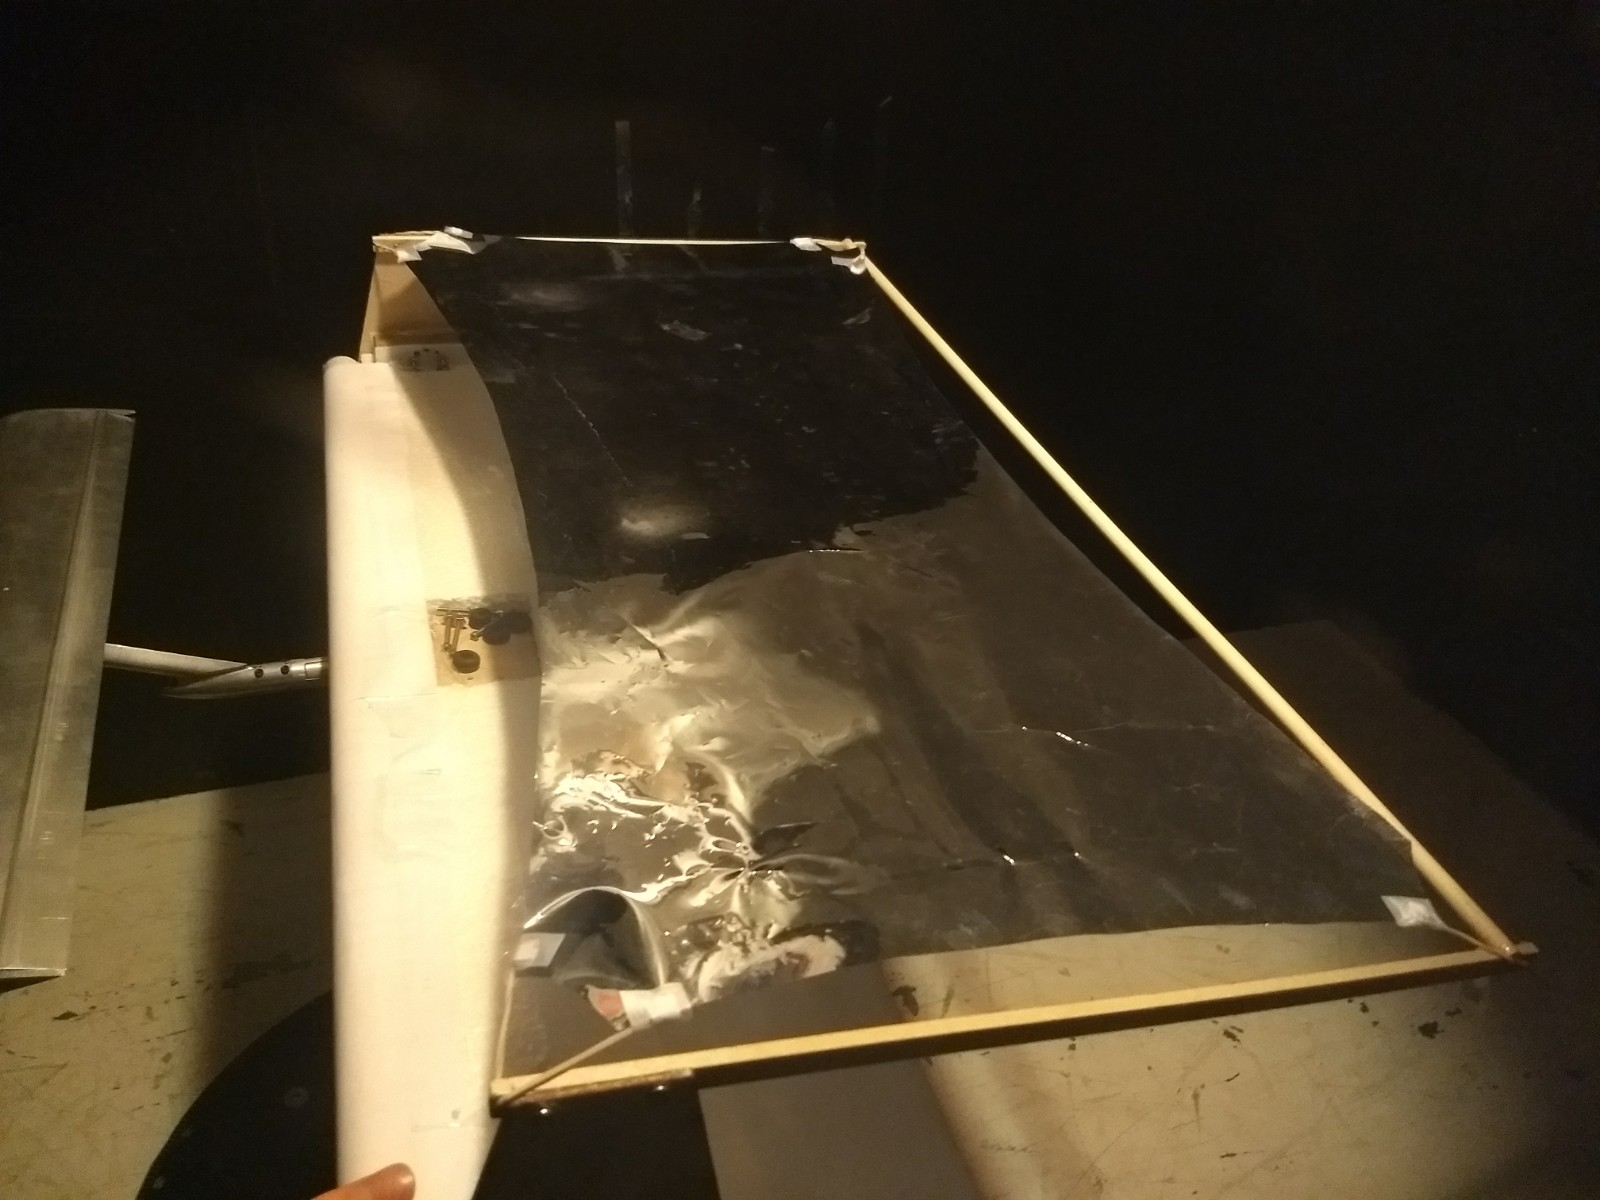
\includegraphics[width = 0.6\linewidth]{with_mylar.jpg}
	\caption{Tension Concept Version 3 in the Wind Tunnel}
\end{figure}

\subsection{Tension Concept Version 4}

Upon further consideration, it appears that previous theories of flutter reduction via tension were inaccurate in that they assumed that
tension (or more precisely, stress) in both lateral and longitudinal directions was important. However, upon observing the flutter in the wind
tunnel, it appears as though the flutter consists of the sheet flexing longitudinally. Thus stress in the longitudinal direction should be the
primary concern for reducing flutter. In light of this theory, TC V. 2/3 was poorly designed. When supporting the sheet from the corners, stress
in the lateral direction flows primarily along the leading and trailing edges, whereas stress in the longitudinal direction flows primarily
along the lateral edges. However, in order to reduce flutter we would like longitudinal stress to be uniformly distributed.

The wire constraint (TC V. 1) model was designed to distribute stress uniformly. However, it was abandoned because loose spots were still
observed. I would like to propose a hypothesis for why this was the case. The wire was taped to the sheet, so the adhesive on the tape
may have exerted a significant friction force on the wire. So, the wire could have exerted considerable force on the sheet in the direction
tangential to its edges, which would in turn cause the distribution of tension along the length of the wire to deviate from the ideal. All
of this would have led to a nonuniform distribution of longitudinal stress in the sheet.

In response to this, a new concept was developed. The wire was replaced by a thread, which had shorter threads knotted to it at regular
intervals. These shorter threads were taped to the sheet such that the main thread is parallel to the leading edge of the sheet, and the
supporting wires are perpendicular, connecting the main thread to the sheet. Thus the main thread may undergo small tangential movements while
exerting minimal tangential force on the sheet. Furthermore, by observing the orientation of the supporting wires, it can be verified that
the tangential force is small compared to the normal force.

\subsection{Tape Concept}

All of this research has been based on the theory that the sheet will vibrate in any places where it is unconstrained, i.e. the tension
in the sheet is zero. In the Tension Concept series of prototypes, the sheet was placed under tension by connecting it to stretched
rubber bands. However, it was hypothesized that by taping the sheet to the fram along its lateral edges in such a precise manner that there
were no "loose" spots, i.e. locations where there was excess material, allowing the sheet to deflect without becoming taut, then when the sheet
begins to generate lift, the upward pressure will cause a considerable tension force everywhere in the sheet, preventing it from vibrating. Thus,
the Tape Concept model was built identical to TC V.4 (including the concave parabolic leading and trailing edges) except without the threads on
the leading and trailing edges.

This may be undesirable to use on an actual aircraft, because of the structural complexity required to constrain the sheet at all points along
its lateral edges. Nonetheless, it is beneficial to know if this method is effective, in case a convenient way of implimenting it on an actual
aircraft is discovered.

\subsection{Tension Concept Version 5}

It was hypothesized that taping the sheet along its lateral edges in TC V.4 may not be necessary in order to prevent the sheet from flexing upward
due to its own lift. Because the threads are under high tension, it will likely take a very large force to stretch them upward. Therefore, TC V.5
was built using a sheet suspended by rubber bands as in TC V.3, except with threads along its leading and trailing edges, as in TC V.4.

In previous models, there has been some play in the connection between the sheet and the wing, so the angle of attack of the sheet with respect
to the wing cannot be determined precisely, but it was between 0 and 5 degrees. In TC V.5, the sheet was fixed at $3.5\degree$ higher AOA than
the wing.

\begin{figure}
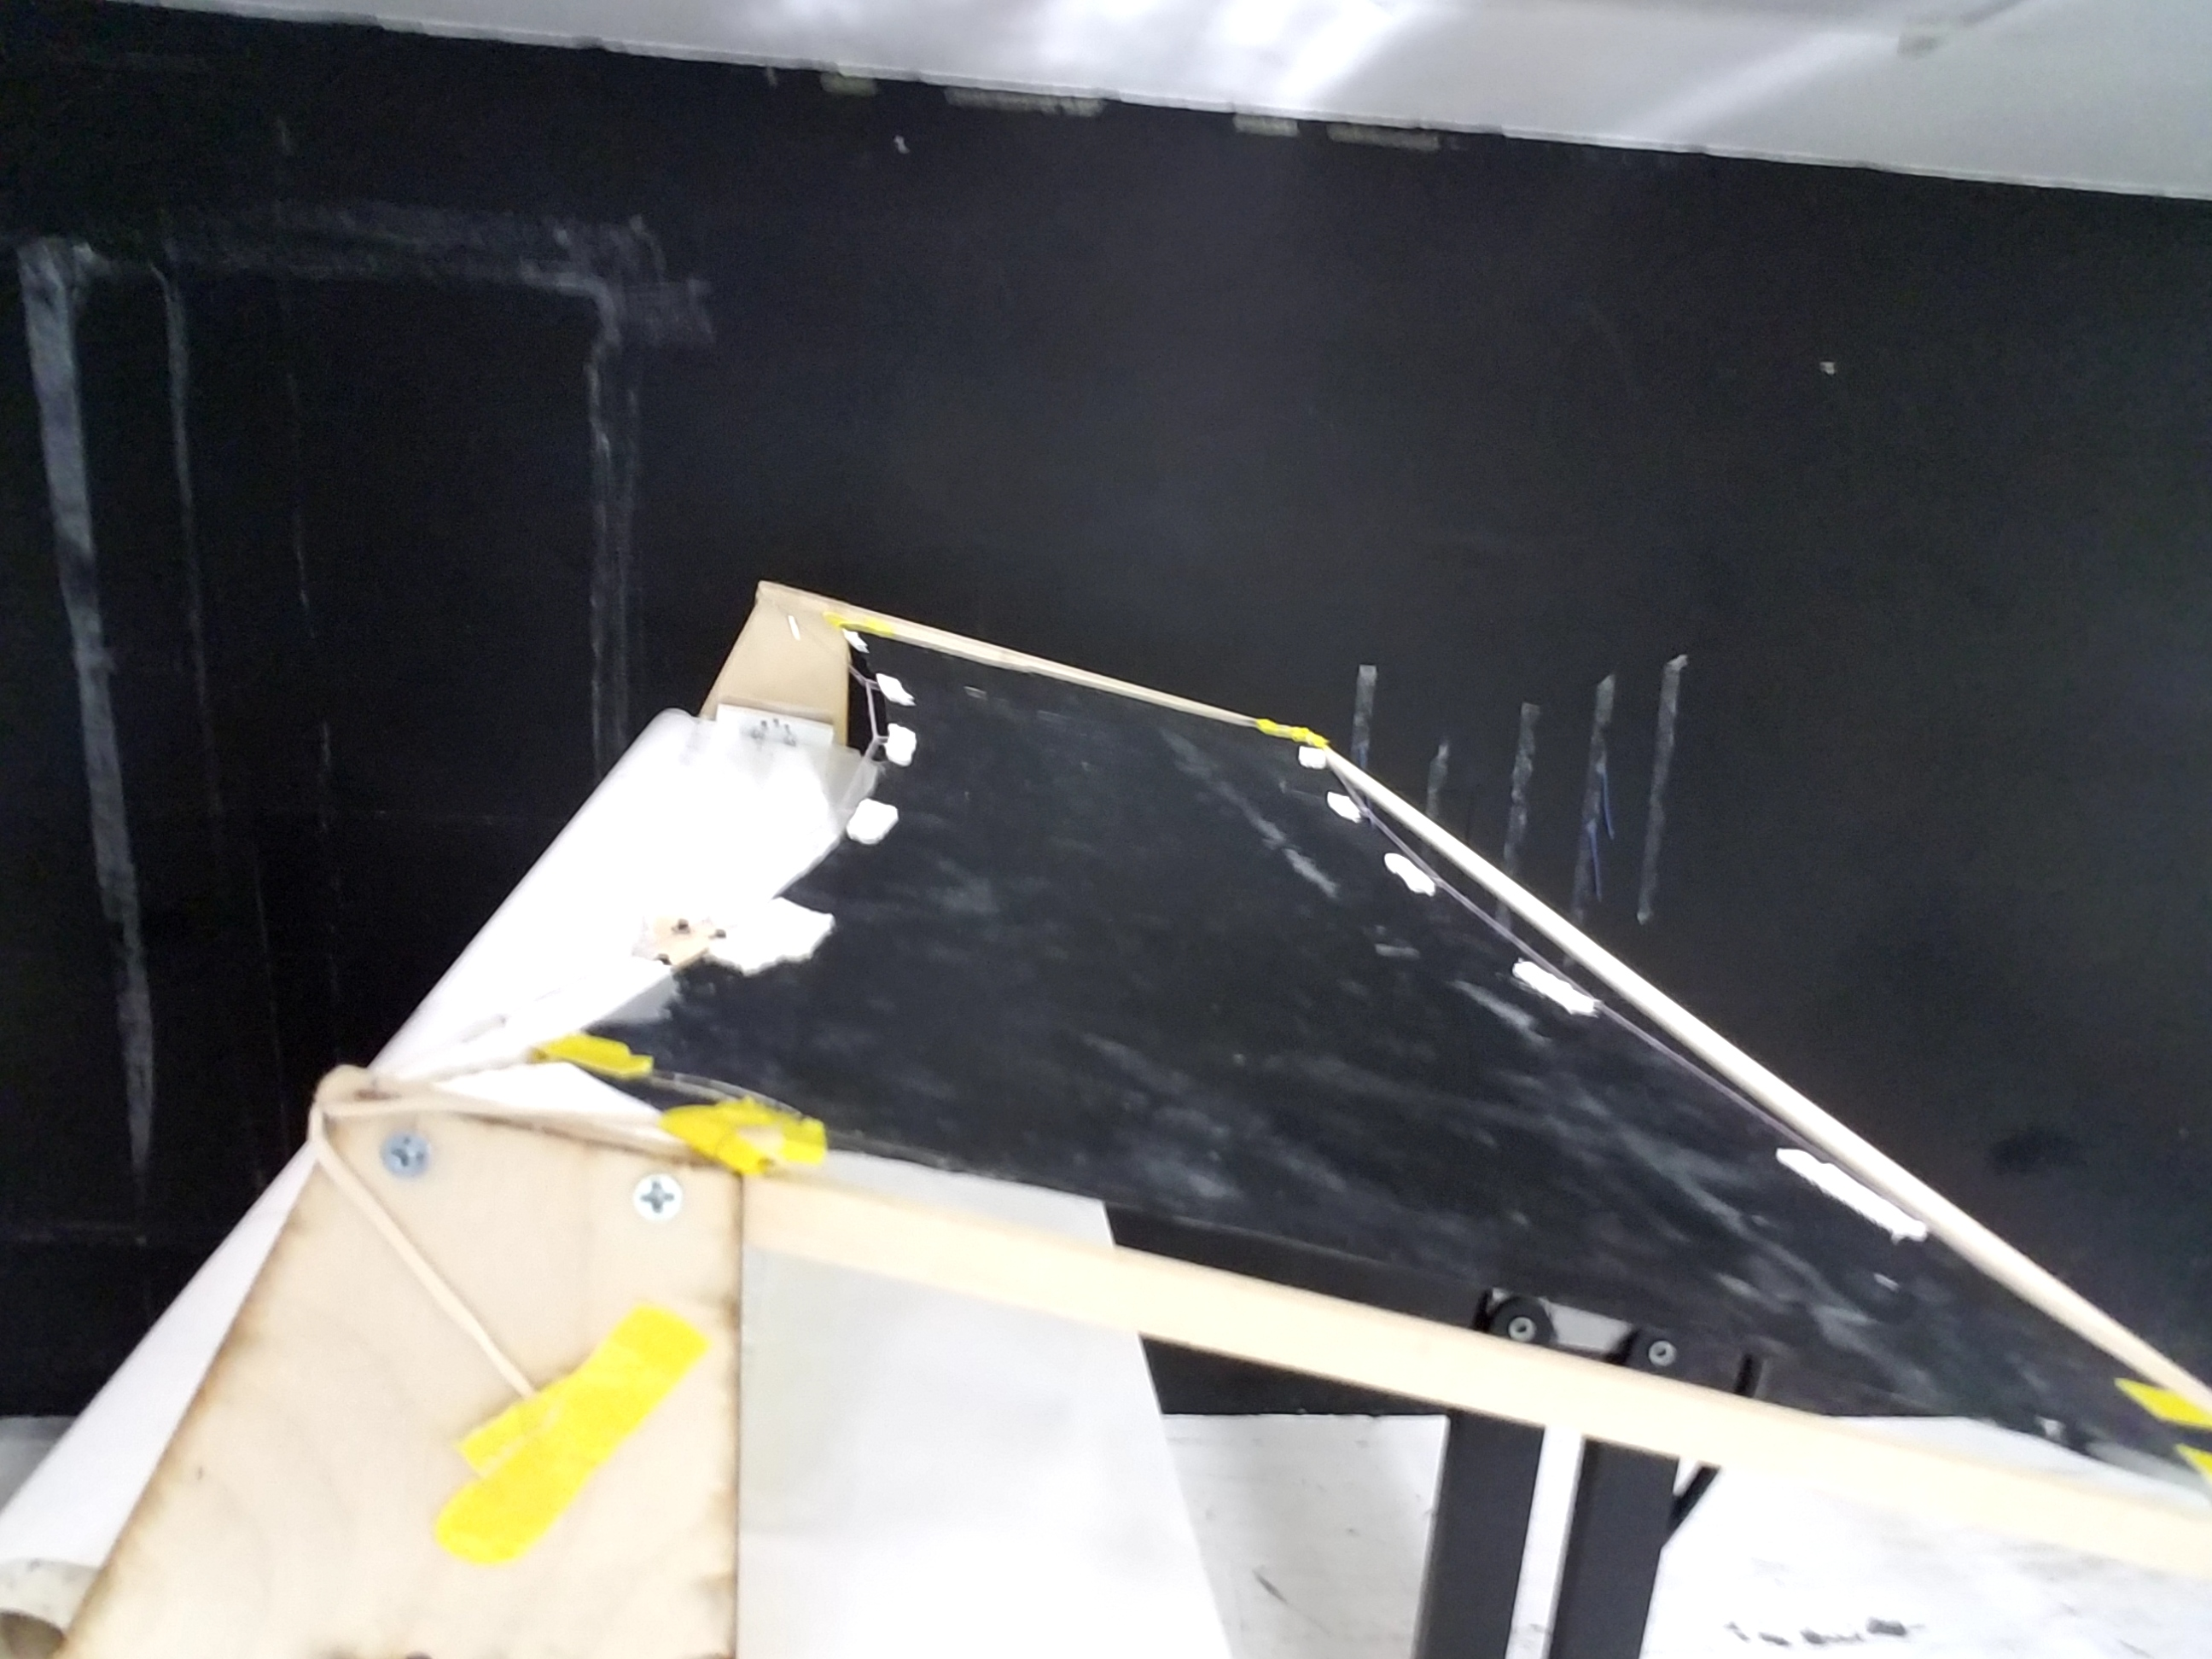
\includegraphics[width = 0.5\linewidth]{tcv5.jpg}
\caption{TC V.5 in the wind tunnel}
\label{tcv5}
\end{figure}


\subsubsection{Fan blade}
In order for the experimenters to gain experience using the wind tunnel, a test will be run on a fan blade.  The dimensions of the fan blade
were measured
and a CAD (SOLIDWORKS) file created.  It will be taken to the machine shop and some holes will be drilled in it in order that it may be
bolted to the load cell mount.

The fan blade is a flat plate.  It's planform is approximately rectangular, except that its two shorter edges are curved with constant
radius.  It's area is $0.06153m^2$, span is 525.8mm, and chord is 120.7mm.

\begin{figure}
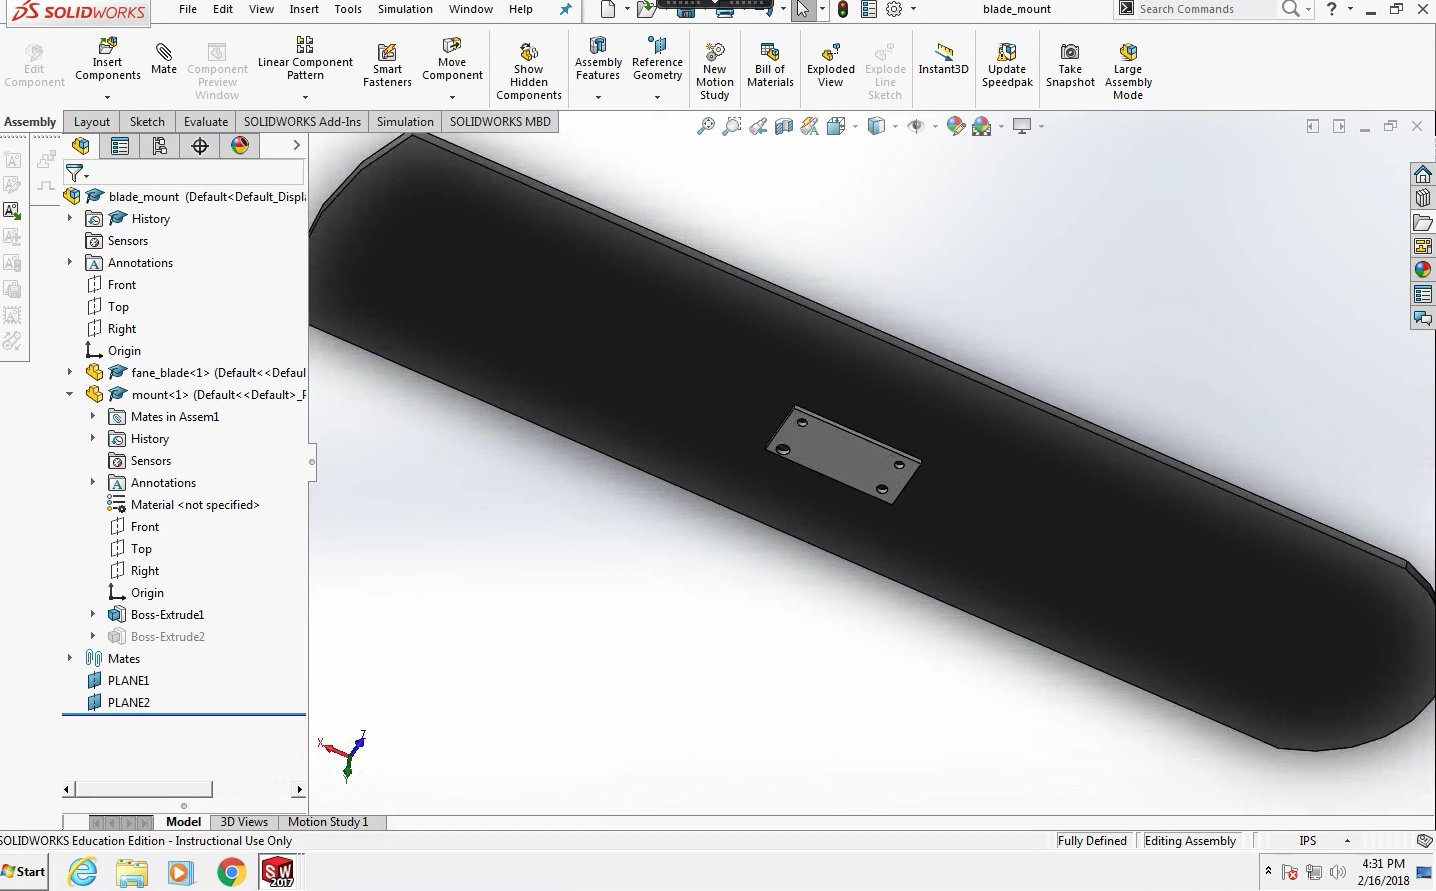
\includegraphics[width = 15cm]{blade_CAD.png}
\caption{The blade in position over the load cell mount in CAD}
\end{figure}

\subsection{Load cell details}

\subsubsection{Custom Mount}

For the earlier models (up through TC V.3) the following load cell was used. It was problematic in that reliable drag measurements
could not be obtained.

The single strut mount in the Low Turbulence wind tunnel was assessed.  Measuremeants of its mounting holes and other primary features
were taken, and a CAD (SOLIDWORKS) model was created.  An engineering drawing was produced in order that the models may be effectively
fitted to it.

The load cell was calibrated by applying known loads to it and measuring the strain gauge voltages.  It was assumed that
\[
\begin{bmatrix}
L_V & D_V
\end{bmatrix}
\begin{bmatrix}
A & C\\
B & D
\end{bmatrix}
=
\begin{bmatrix}
L & D
\end{bmatrix}
\]
where $L_V$ and $D_V$ are the voltage readings from the strain gauges and L and D are the lift and drag, for some coefficients A, B, C,
and D.  Using dataset on the order of 10 readings and a least squares approximation, the coefficients were found to be

\begin{tabular}{c|c}
A & 7.57\\
B & 1.50\\
C & 1.30\\
D & 1.33
\end{tabular}

The wind tunnel was run in order to find the lift and drag of the mount.  At each velocity, a series of readings was taken within
a few seconds, and the mean and standard deviation were found.  The values at 16m/s are quoted here.  Velocity is in m/s and force
is in N.
\begin{tabular}{c c c c c}
$U_\infty$ & Lift & std(Lift) & Drag & std(Drag)\\
16 & -0.6304 & 0.05194 & 0.809 & 0.02220
\end{tabular}

\subsubsection{Sting Mount}

For later models (TC V.4 and later), a sting mount which is more reliable than the custom mount was used. It reliably gives normal and
axial force measurements which may be converted to lift and drag measurements.

\subsection{Static testing of the model}

\subsubsection{Simple Version}
The sheet was unstable.  The leading edge had a tendency to fold up,
but could be induced to fold down by changing the AOA.  It was observed that there was a prominent crease in the sheet near
the leading edge, caused by the manner in which it was stored prior to being used as a construction material.  The spot in which
the sheet bent due to the instability coincided with the crease, leading the experimenters to conclude that the crease caused the
instability.  The amount of flutter was small at negative AOA, moderate at very high AOA, and extreme at AOA close to zero.

\subsubsection{Dampening Holes}
The holes caused no difference which was visually apparent.

\subsubsection{Wire Constraint}
The amplitude of the flutter was reduced to a fraction of its original value, however it was still present.  Similar to the former two
test cases, the flutter was smallest at negative AOA, and highest at small AOA, and moderate at high positive AOA.

\subsubsection{Fan Blade}
The following lift and drag curves, and drag polar, were obtained:

\begin{figure}
	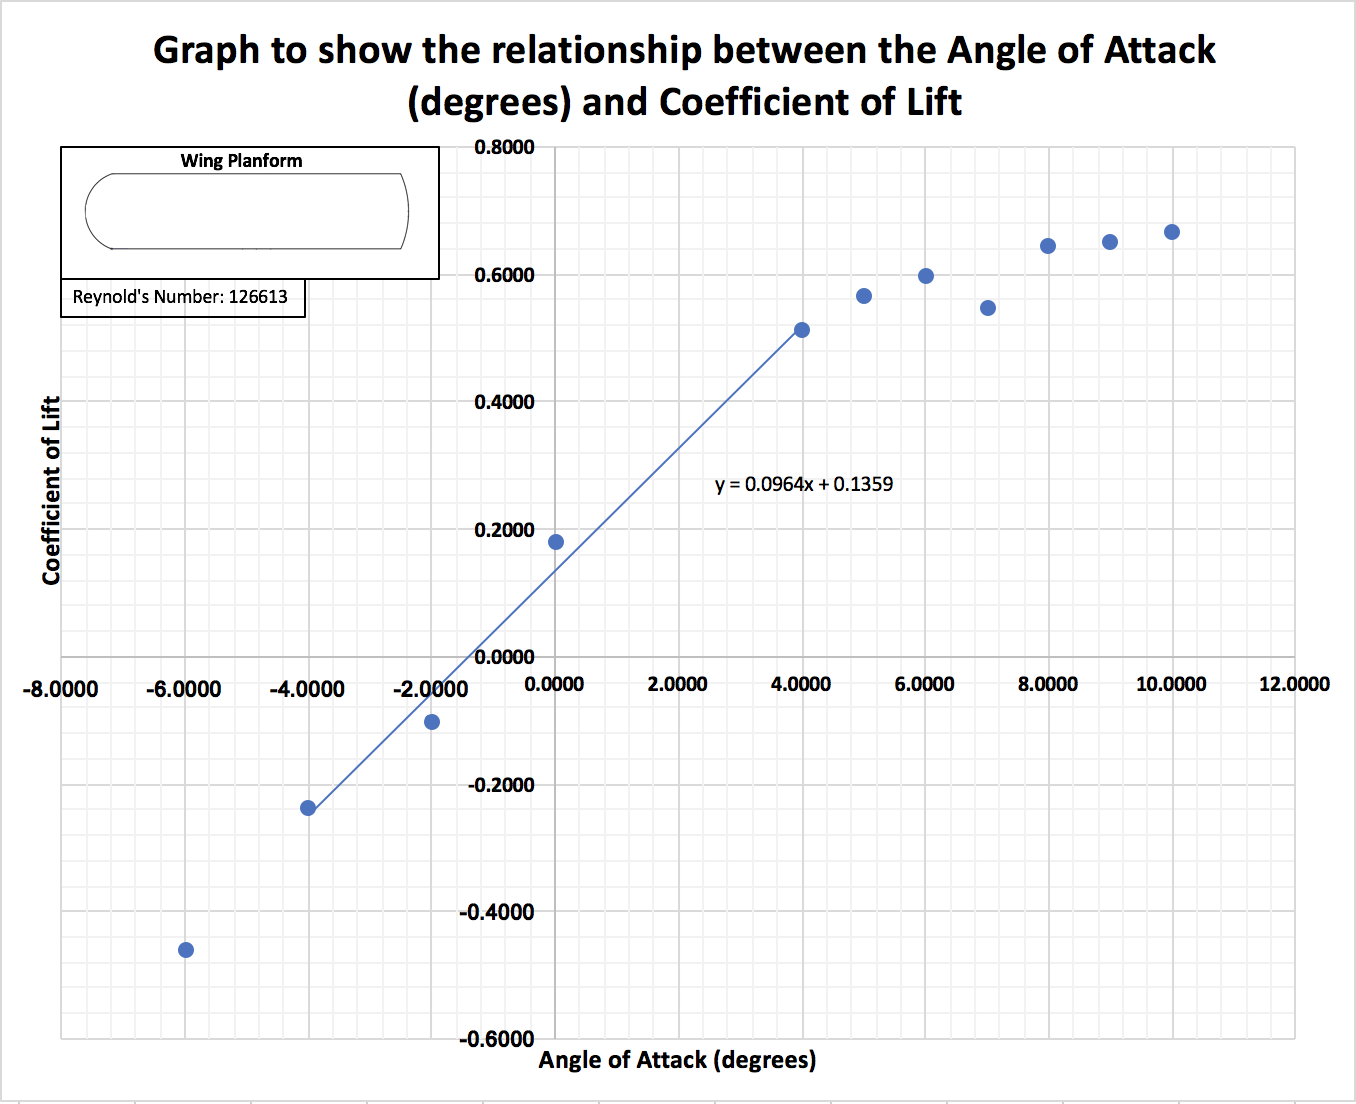
\includegraphics[width = 0.5\linewidth]{AOA_Cl.png}
	\caption{Lift curve for fan blade}
\end{figure}
\begin{figure}
	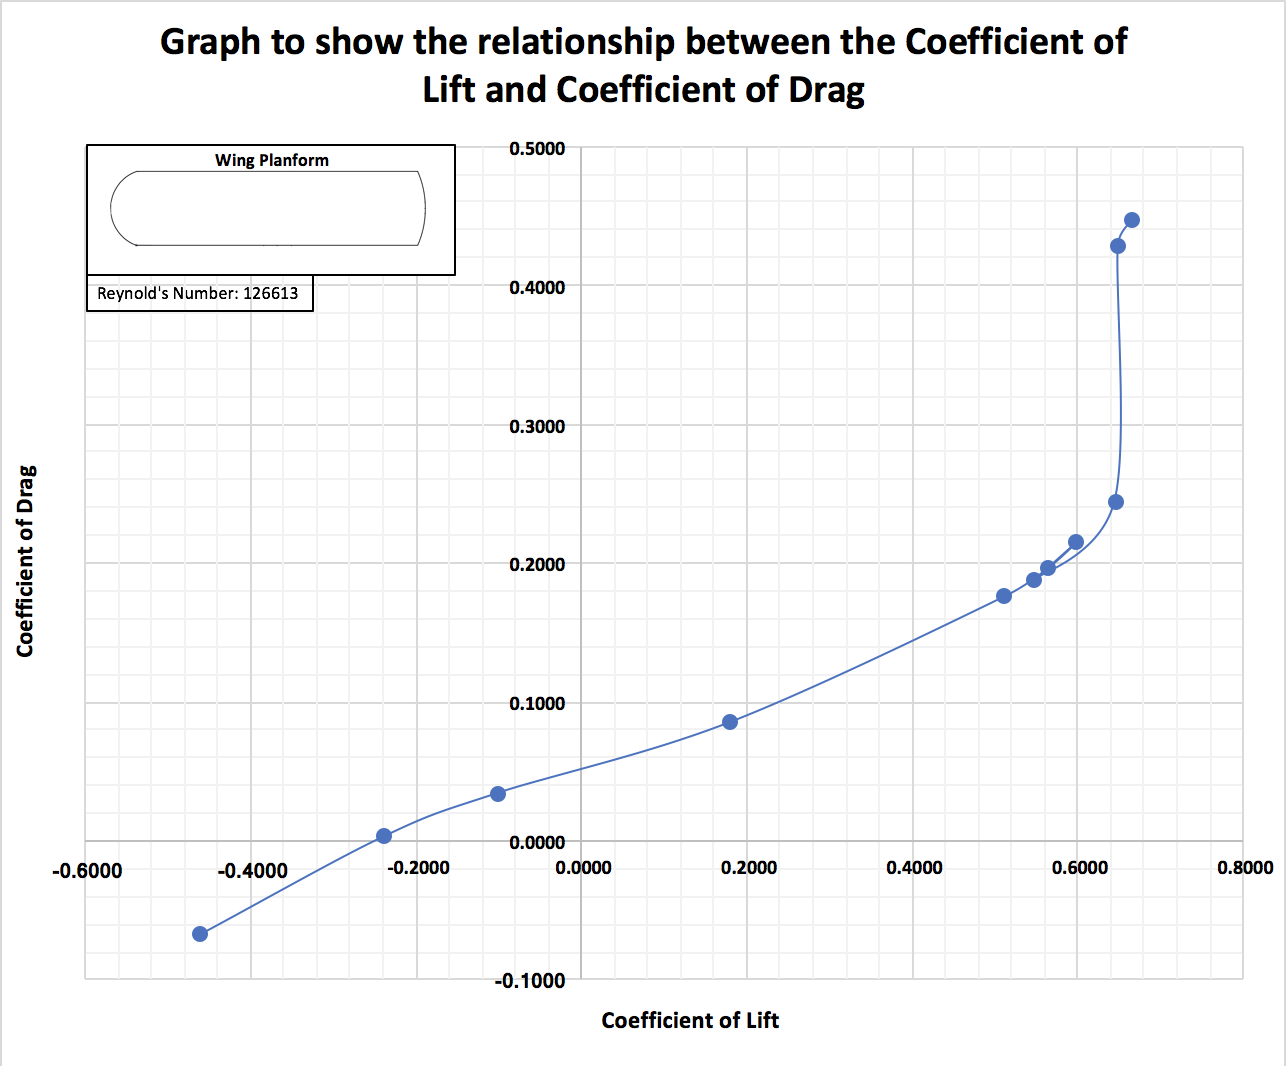
\includegraphics[width = 0.5\linewidth]{Cl_Cd.png}
	\caption{Drag polar for fan blade}
	\label{fan blade data}
\end{figure}

The lift curve slope was calculated (in radians) to be 5.6.  When compared to the value of $2\pi$ predicted by Thin Airfoil Theory,
this produces an error of 11%.

\subsubsection{Tension Concept v2}
The model was tested and lift measurements were taken (drag measurments could not be obtained because of a problem with the load
cell calibration).
At higher AOA, the sheet stretches upward, increasing the geometric angle of attack of the middle region of the sheet more than the change
in the base which was manipulated. This billowing is undesirable because it decreases the reflector area and interferes with the lift distribution
in addition to making the lift measurements less meaningful.

The lift-weight stability theory was disproved.  There was noticeable amounts of flutter, even at reasonably high AOA. The sheet had an undesirable
tendency to bow upward at high AOA and high speed and downward at low AOA and low speed, the flutter was present at all reasonable AOA values.

The lift-curve-slope for the plastic sheet was calculated to be 3.19, although the error margin of the data renders our confidence in this number
very low. The lift data for the plasit sheet is plotted below. The error bars represent the standard deviation of the data readings as they were
collected.

\begin{figure}
	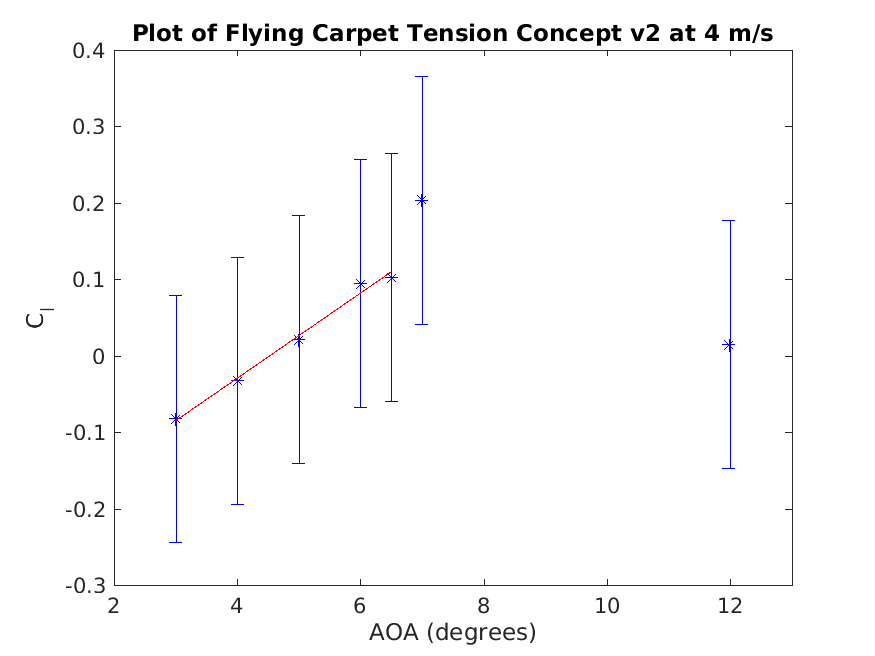
\includegraphics[width = 0.6 \linewidth]{tension_model_lift.png}
	\caption{Lift data for TC V.2}
	\label{tcv2}
\end{figure}

\subsection{Tension Concept V.3}

Visual inspection indicated that the mylar sheet fluttered with greater amplitude than the plastic one.

\subsection{Tension Concept V.4}

Visual inspection indicated that the flutter amplitude was considerably reduced from TC V.2 and 3.

\subsection{Tape Concept}

Visual inspection indicated that the flutter amplitude was roughly equal to that of TC V.4.

\subsection{TC V.5}

Visual inspection indicated that the flutter amplitude was roughly equal to that of TC V.4. After this was observed, the speed was increased
to 10 m/s, which is a higher speed than any of the other models were exposed to. At that point, the sheet began to flutter violently.
Lift and drag measurements were obtained for
the wing with the sheet removed, and with the sheet on, at two different Reynolds numbers (\ref{tcv5 cl} and \ref{tcv5 dp}). Note that
these are for a finite
wing, so indiced drag is present. Also, the model has many external features, such as fasteners and perforations, which will generate drag and
will not be present on an actual aircraft. Finally, note thati the coefficients were nondemensionalized in terms of the wing, which was 71cm
span by roughly 20cm chord.

\begin{figure}
	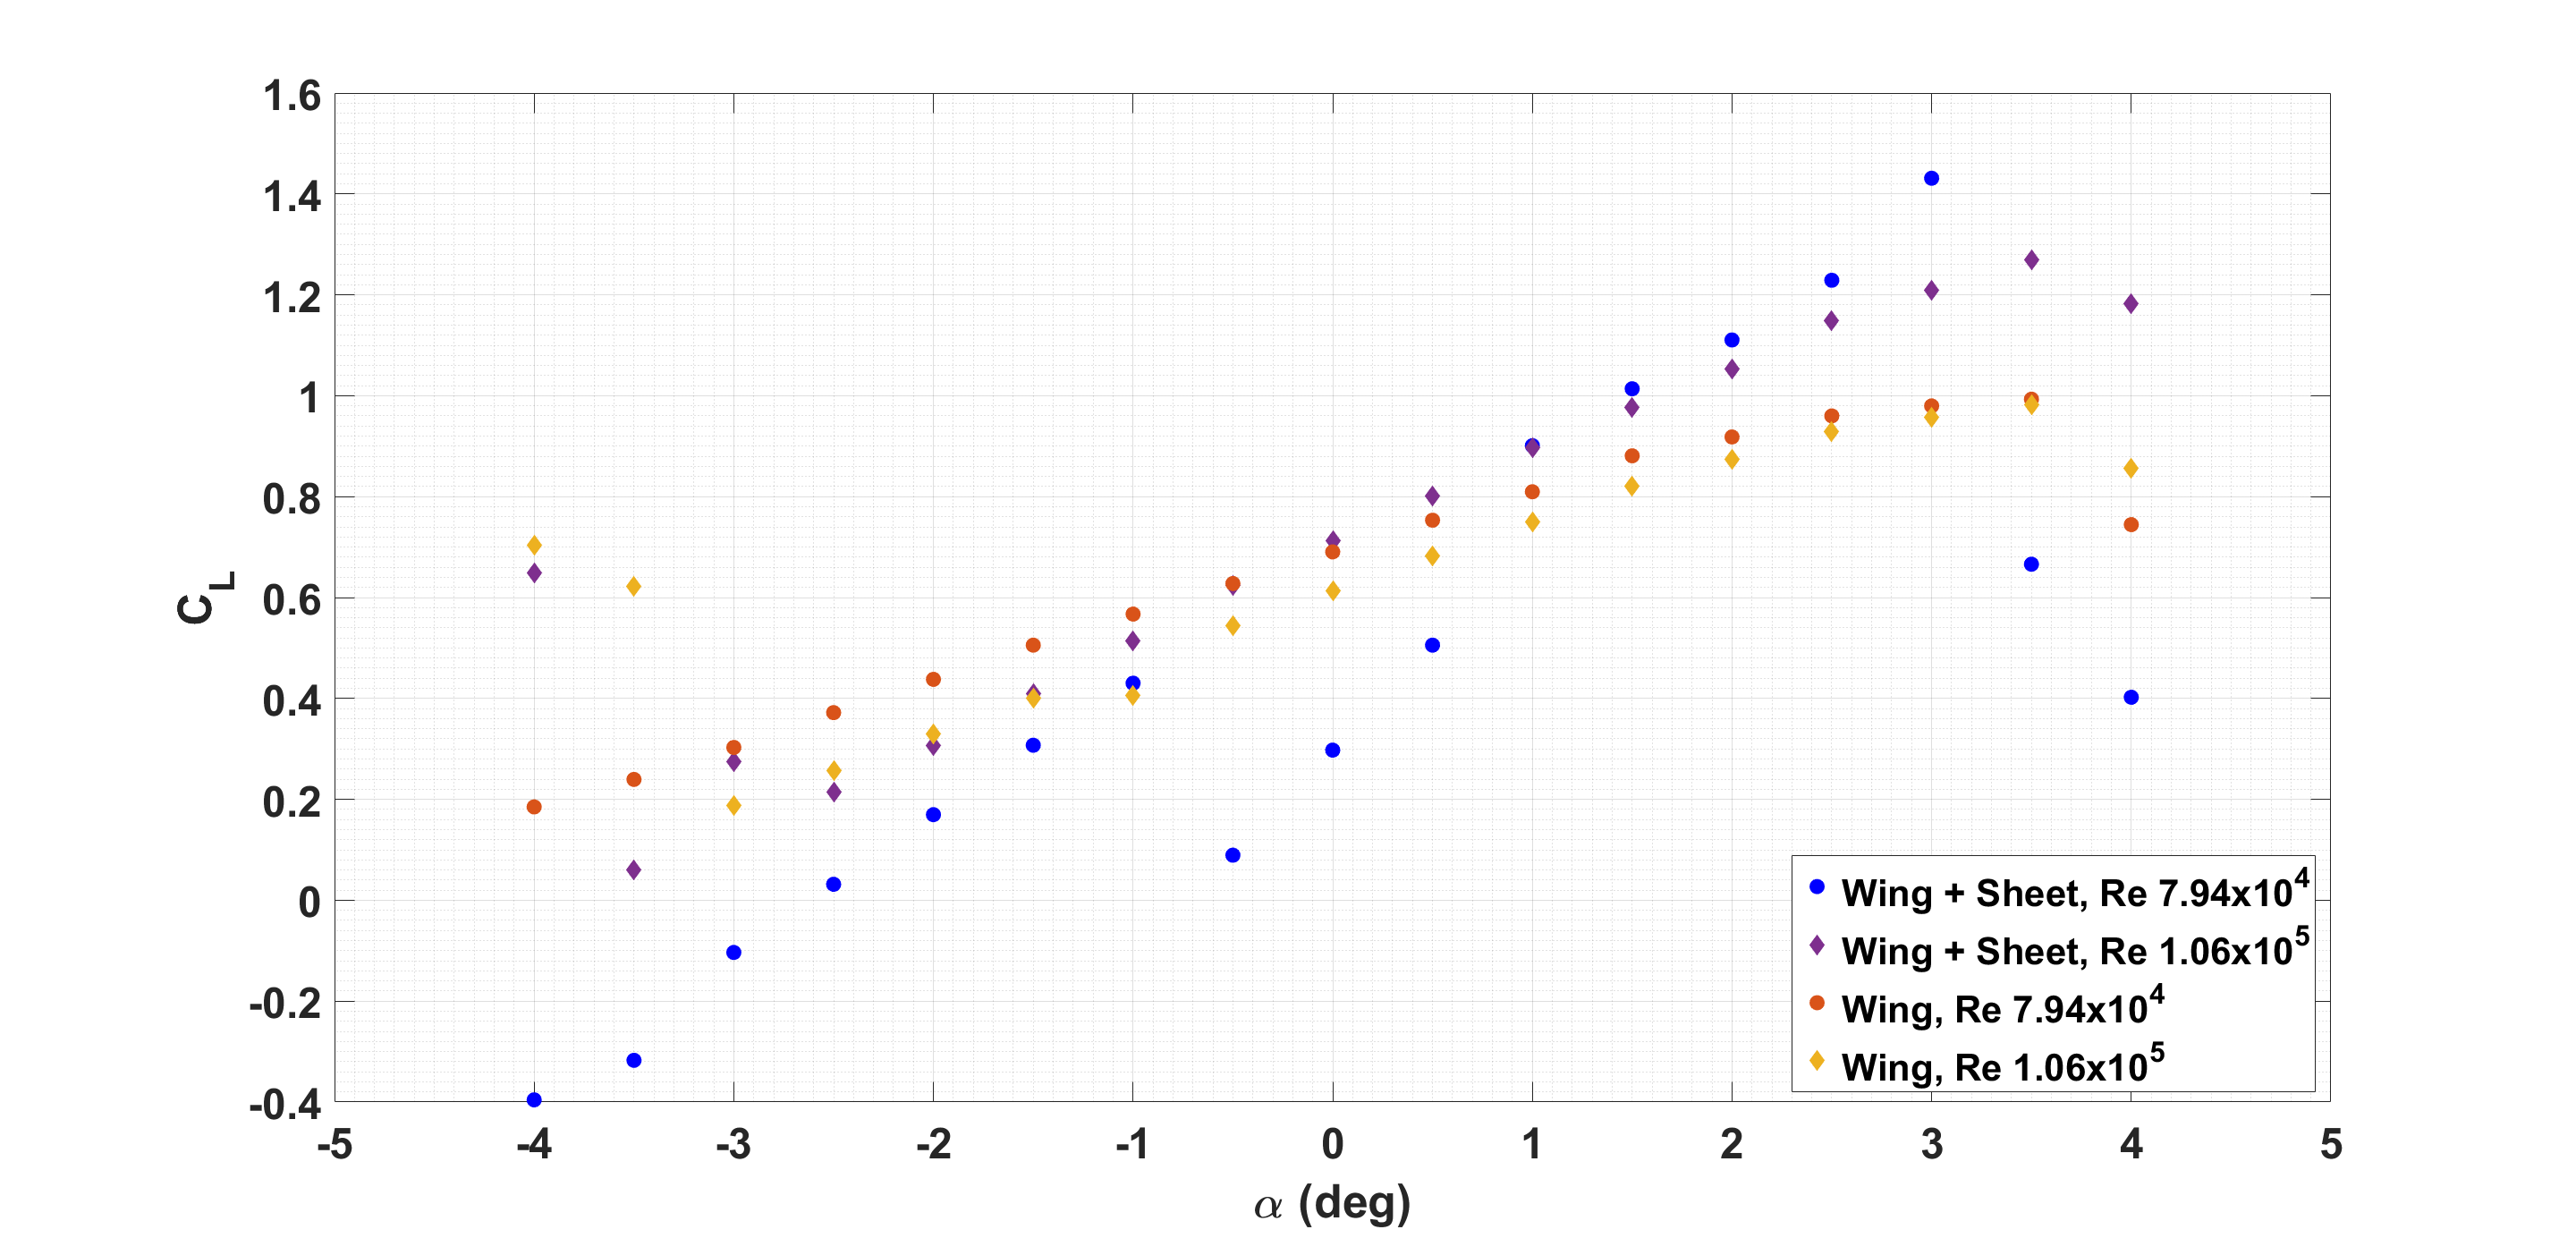
\includegraphics[width = 0.5\linewidth]{tcv5_cl.png}
	\caption{Lift curves for TC V.5}
	\label{tcv5 cl}
\end{figure}
\begin{figure}
	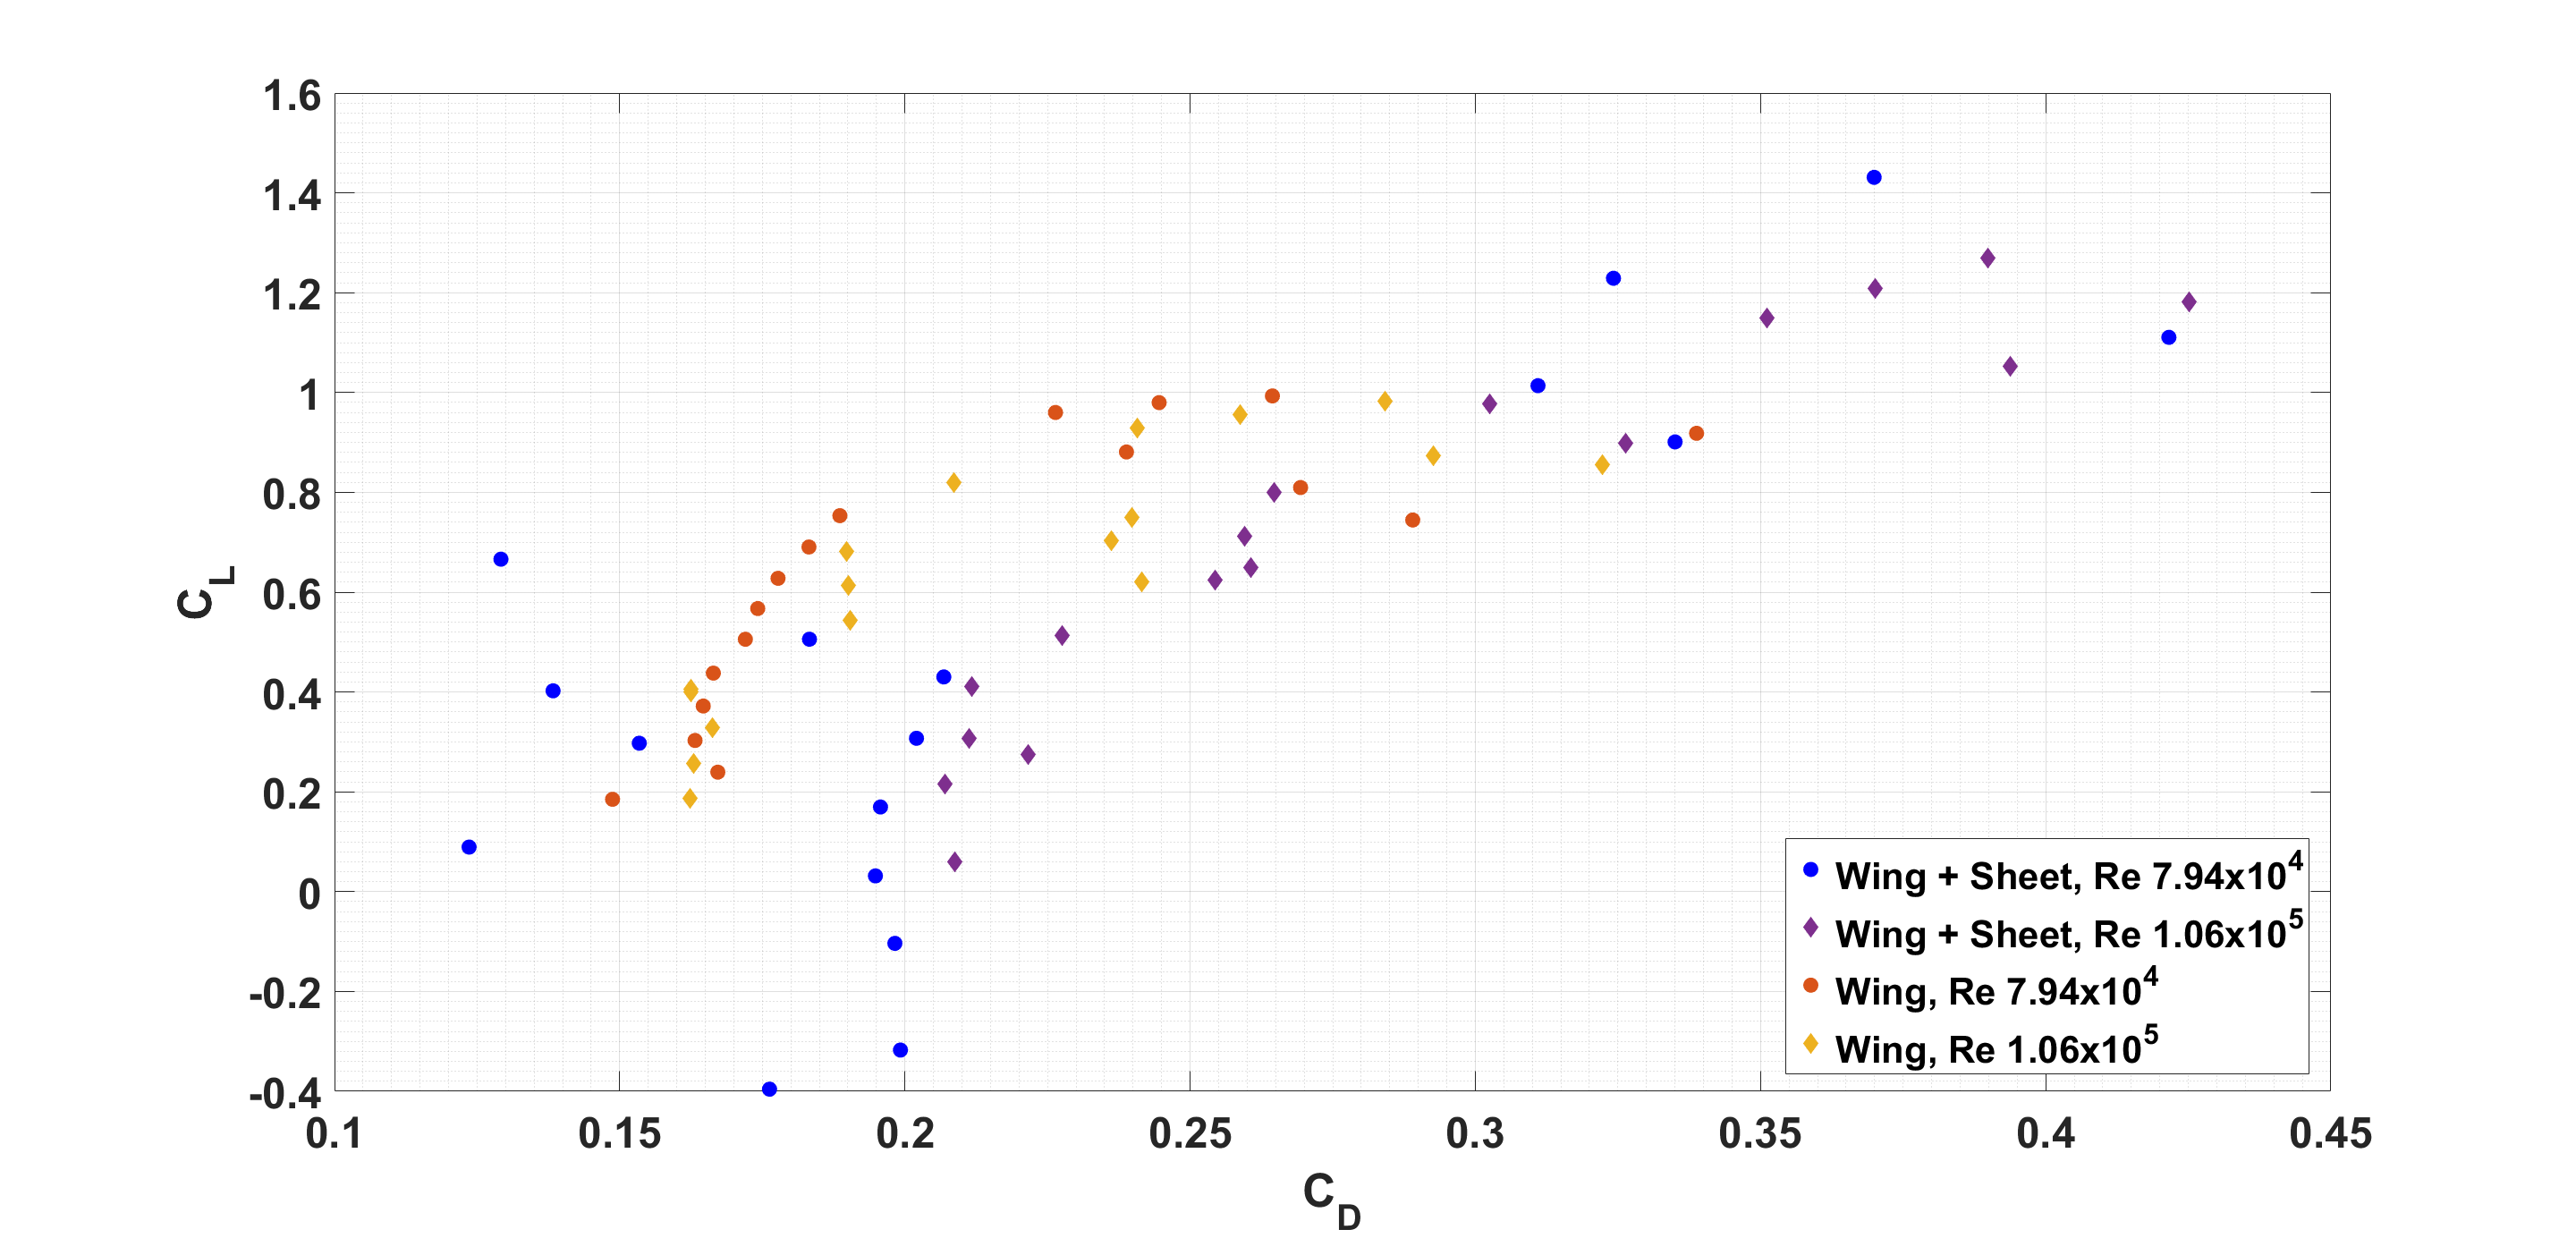
\includegraphics[width = 0.5\linewidth]{tcv5_dp.png}
	\caption{Drag polars for TC V.5}
	\label{tcv5 dp}
\end{figure}

\chapter{Flow and Test Conditions}
\subsection{Preliminary Testing}
The ventilation fan in the wind tunnel was run and the doors to the lab were opened, forming a gentle breeze in the doorway to the wind
tunnel.  The model was held in this wind at various angles of attack.

\subsection{Flat Plate}
The fan blade was tested in the Low Turbulence wind tunnel.  It's lift and drag were measured at 16m/s, and the mount's lift and drag
was subtracted off.  $C_L$ and $C_D$ were calculated using the air density that day and the blade's area (no attempt was made to
calculate the induced drag).

\subsection{Measurement Testing}
After the "open door" test, the model was tested in the academic "Low Turbulenc Wind Tunnel". Tests were usually run at $V_\infty < 8m/s$ in
order to prevent structural failure of the model.

\chapter{Discussion}

So far, the there appear to be two most successful ways to reduce flutter. One is to pull it taut and secure it continuously along its lateral
edges, and the other is to support it under tension using elastic bands at its corners and some form of cable along its leading and trailing
edges, which should be on concavely parabolic shape. Furthermore, care must be taken in order to ensure that the force the cable exerts on
the sheet is in a purely longitudinal direction, i.e. there is not a large tangential component due to friction. Both these methods may be
used in tandem, but there is little, if any, additional benefit. In addition to the discovery of these methods,
it appears that the sheet will flutter less with decreasing Reynolds number.

Lift and drag were obtained for a sheet using the cable method of flutter reduction. Even when accounting for induced drag, the drag seemed quite
high, although this may be due to parasite drag from unnecessary external fixtures. Further testing with a higher quality model is required
in order to get meaningful drag data. Also, tests involving different wing chord and angle of incidence with respect to the sheet should be
conducted in order to understand the interactions between these two components.

\begin{thebibliography}{9}
\end{thebibliography}


\end{document}
